\documentclass[tikz,convert={outfile=images/tr-graph.png,density=1000}]{standalone}
\usepackage[build={latexoptions={-output-directory=latex/png}}]{standalone}
\tikzset{
  ->/.style={draw=white!50!black,-stealth}
}
\tikzstyle{every node}=[color=white!50!black,font=\footnotesize]
\begin{document}
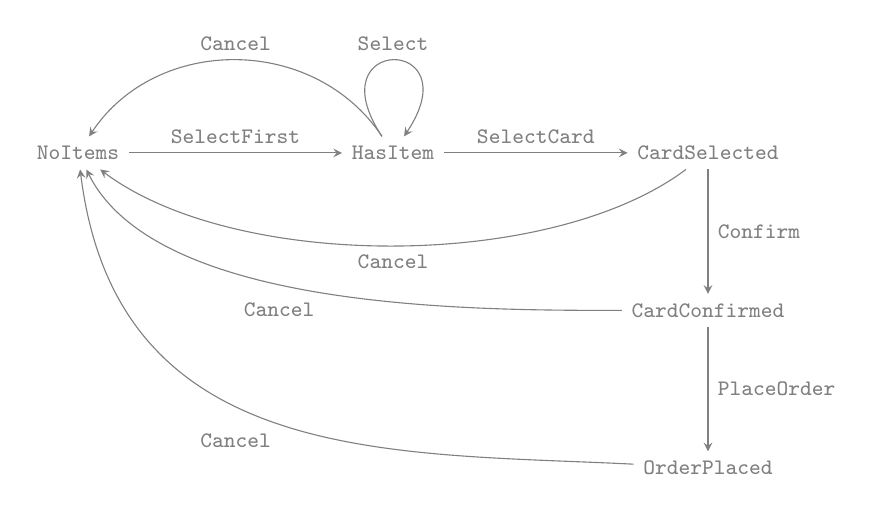
\begin{tikzpicture}
    \node (A) at (0,0) {\texttt{NoItems}};
    \node (B) at (4,0) {\texttt{HasItem}};
    \node (C) at (8,0) {\texttt{CardSelected}};
    \node (D) at (8,-2) {\texttt{CardConfirmed}};
    \node (E) at (8,-4) {\texttt{OrderPlaced}};
    \draw[->] (A) -- node[above]{\texttt{SelectFirst}} (B);
    \draw[->] (B) .. controls (3,1.5) and (5,1.5) .. node[above]{\texttt{Select}} (B);
    \draw[->] (B) .. controls +(-1,1.5) and +(1,1.5) .. node[above]{\texttt{Cancel}}  (A);
    \draw[->] (B) -- node[above]{\texttt{SelectCard}} (C);
    \draw[->] (C) .. controls +(-2,-1.5) and +(2,-1.5) .. node[below]{\texttt{Cancel}}  (A);
    \draw[->] (C) -- node[right]{\texttt{Confirm}} (D);
    \draw[->] (D) -- node[right]{\texttt{PlaceOrder}} (E);
    \draw[->] (D) .. controls +(-3,0) and +(1,-2) .. node[below left]{\texttt{Cancel}} (A);
    \draw[->] (E) .. controls +(-4,0.2) and +(0.5,-4) .. node[below left]{\texttt{Cancel}} (A);
\end{tikzpicture}
\end{document}
